\section{Routing Mechanism and Quality--Compute Frontier}

The Qwen routing lane is the cleanest explanation for why training-free
anti-recomputation can work at all. It tells us what kind of temporal signal
is useful, what kind is too blunt, and where the semantic-substitution story
stops.

\subsection{Clean-Tree Holdout Frontier}

On TOMATO motion, the clean base policy matches dense-8 accuracy while spending
only 3.55 effective fresh frames instead of 8.0. On MVBench motion, the same
clean base policy reaches a higher point estimate than dense-6 while spending
less visual refresh: 0.600 accuracy at 4.06 effective fresh frames versus
0.567 at 6.0 fresh frames. At \(n=30\), that is a pointwise Pareto frontier
observation, not a statistical victory lap. Those are not wall-clock claims.
They are benchmarked statements about preserved answer quality at lower
effective visual budget.

\subsection{Automated Snapshot}

\IfFileExists{generated/tables/lane_a_holdout.tex}{
\begin{table}[H]
\centering
\caption{Audited Qwen holdout frontier. The higher-stability MVBench refinement is discussed in text but not plotted.}
\label{tab:lane-a-holdout}
\small
\renewcommand{\arraystretch}{\PaperTableStretch}
\begin{tabular}{lllrrrl}
\toprule
Benchmark & Policy & Relation & Acc. & Fresh & Comparator & Comparator acc. \\
\midrule
TOMATO & planner base & tie & 0.333 & 3.55 & dense-8 (8) & 0.333 \\
MVBench & planner base & frontier & 0.600 & 4.06 & dense-6 (6) & 0.567 \\
\bottomrule
\end{tabular}
\end{table}

}{
\draftnote{Run \texttt{make paper-sync} to generate the automated holdout table.}
}

\begin{figure}[H]
  \centering
  \IfFileExists{generated/figures/lane_a_pareto.pdf}{
    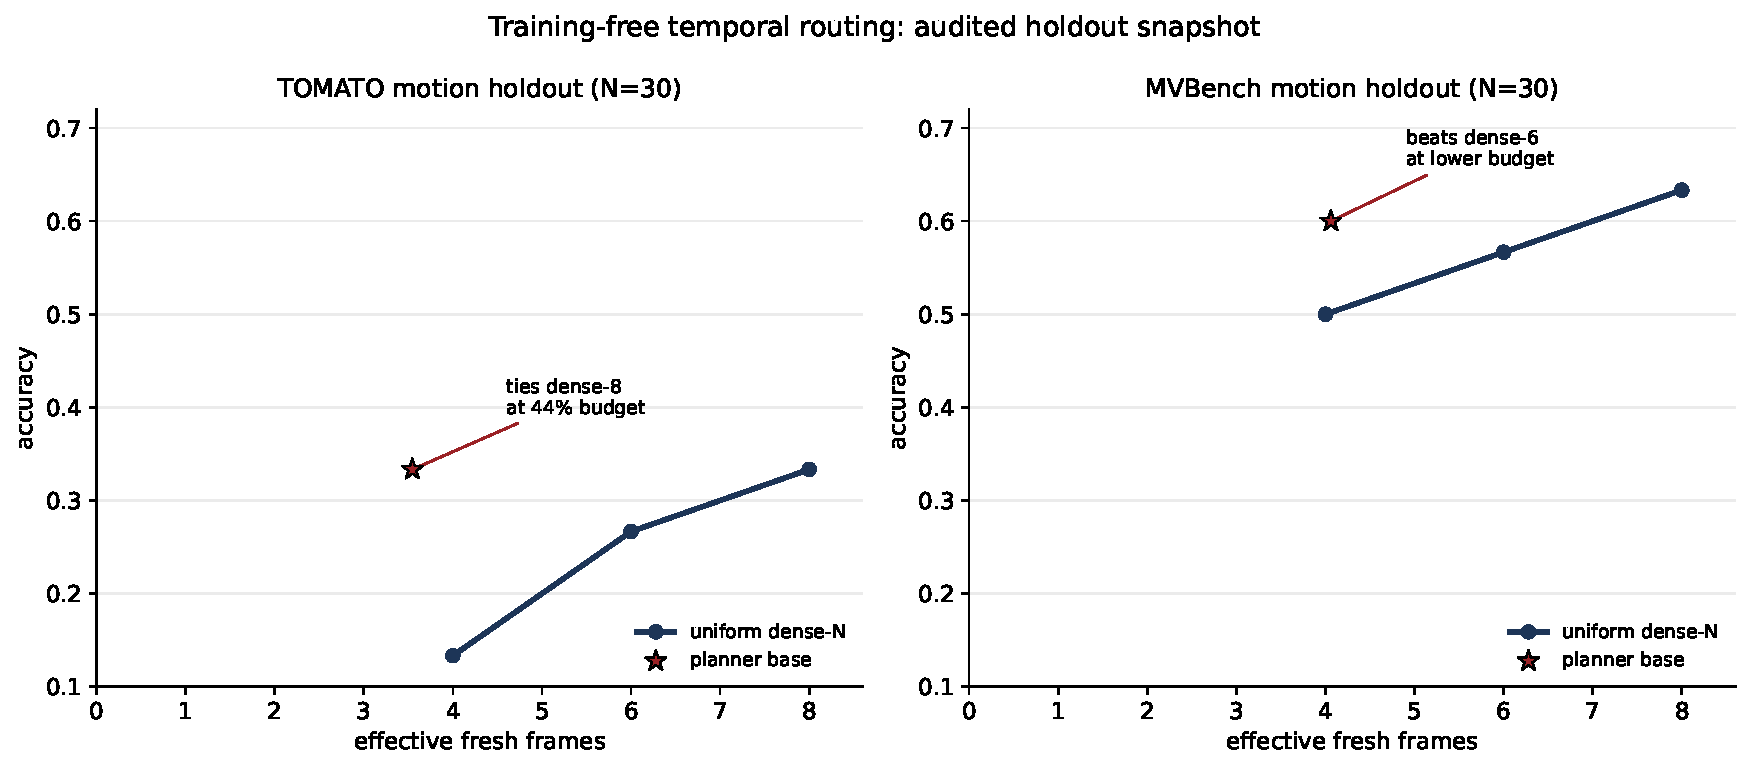
\includegraphics[width=\linewidth]{generated/figures/lane_a_pareto}
  }{
    \fbox{\parbox{0.9\linewidth}{Run \texttt{make paper-sync} to generate the Lane A Pareto figure.}}
  }
  \caption{Clean-tree Qwen holdout frontier from canonical artifact summaries.
  The automated manuscript snapshot intentionally excludes the MVBench
  \texttt{sticky4} variant because the current artifact is dirty-tree and
  remains supplementary until rerun clean.}
  \label{fig:lane-a-pareto}
\end{figure}

The omitted MVBench \texttt{sticky4} refinement remains scientifically
interesting: it reaches 0.633 accuracy at 4.49 effective fresh frames and
therefore matches dense-8 at 56\% of the fresh-frame budget. The current
artifact is still dirty-tree, so the default manuscript snapshot keeps it out
of the main figure on purpose.

\subsection{Novelty Magnitude Alone Is Not Enough}

The most important baseline in this repo is not another cached policy; it is a
non-cached novelty-ranked dense baseline. This baseline asks whether the cached
planner is merely doing smart frame selection in disguise. It is not.

\begin{table}[H]
\centering
\caption{Novelty-ranked dense baseline imported from the phase~1.34 note. This
table is still hand-carried from the authoritative note because a stable
checked-in artifact path for these summaries has not yet been wired into
\texttt{paper-sync}.}
\label{tab:novelty-ranked-dense}
\begin{tabular}{llrr}
\toprule
Benchmark & $N$ & Uniform dense & Novelty-ranked dense \\
\midrule
TOMATO & 4 & 0.133 & 0.133 \\
TOMATO & 6 & 0.267 & 0.167 \\
TOMATO & 8 & 0.333 & 0.233 \\
MVBench & 4 & 0.500 & 0.567 \\
MVBench & 6 & 0.567 & 0.567 \\
MVBench & 8 & 0.633 & 0.567 \\
\bottomrule
\end{tabular}
\end{table}

On TOMATO, novelty ranking hurts once the budget rises above four frames. On
MVBench, it helps at $N=4$ but then saturates and fails to improve with larger
budgets. The cached base policy beats every novelty-ranked dense cell on both
benchmarks. The point is not that novelty is useless. It is that temporal
placement is the real objective, and novelty magnitude alone is a poor proxy
for it.

\subsection{Pixel Statistics Predict Features Only Weakly}

To understand why routing can still work when pixel statistics are crude, we
ran a feature-change oracle that correlates blockwise pixel statistics with
blockwise ViT feature change on cached dense features.

\begin{table}[H]
\centering
\caption{Best point-prediction correlations from the feature-change oracle.}
\label{tab:feature-oracle}
\begin{tabular}{lccc}
\toprule
Benchmark & Best statistic & Pearson $r$ & Spearman $r$ \\
\midrule
TOMATO & mean & 0.233 & 0.177 \\
MVBench & changed-pixel fraction & 0.504 & 0.489 \\
\bottomrule
\end{tabular}
\end{table}

These are weak-to-moderate correlations. That is the point. The best routing
statistic in the planner, \texttt{max\_abs}, is not the best point predictor on
either benchmark. Routing and point prediction are different objectives: the
planner only needs a signal that spends scarce refresh budget in the right part
of the clip often enough to preserve the answer.

\begin{sectiontodo}{Finish the mechanism appendix boundary}
The routing section is now in the right role, but three things still need
cleanup before submission: wire the novelty-ranked dense table to stable
artifacts, either rerun or appendix-ize \texttt{sticky4}, and tighten the
caption language after the final venue template lands.

\textcolor{todoBorder}{Source pointers: \path{paper/claim-matrix.md},
\path{research/experiments/2026/2026-04-15-phase-1_20-tomato-motion-slice-enlargement.md},
\path{research/experiments/2026/2026-04-15-phase-1_21-mvbench-motion-slice-enlargement.md},
\path{research/experiments/2026/2026-04-17-phase-1_34-novelty-ranked-dense.md},
\path{research/experiments/2026/2026-04-17-phase-1_36-feature-change-oracle.md}.}
\end{sectiontodo}
